The closed loop system is shown in Figure~\ref{fig:hw_vtol_system_type_altitude}.
\begin{figure}[H]
   \centering
   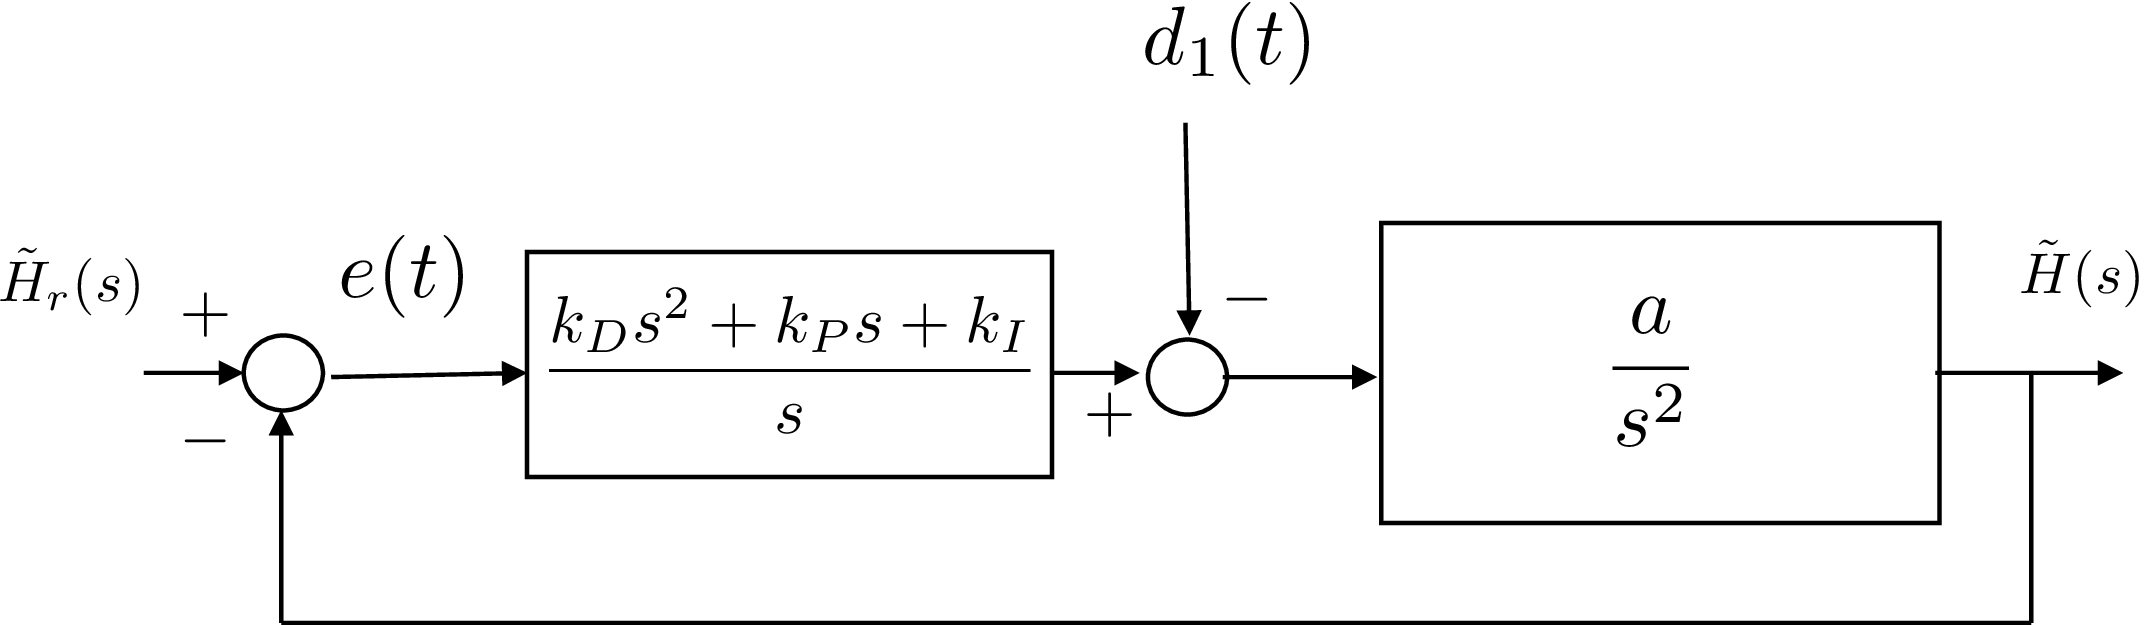
\includegraphics[width=0.7\textwidth]{6_design_studies/figures/hw_vtol_system_type_altitude.pdf}
   \caption{Closed loop system for problem HW~\ref{hw:vtol}.\ref{chap:PID-system-type}.}
   \label{fig:hw_vtol_system_type_altitude}
\end{figure}

The open-loop transfer function is given by
\[
P(s)C(s) = \left(\frac{a}{s^2}\right)\left(\frac{k_D s^2  + k_Ps + k_I}{s}\right),
\]
where
\[
a = \frac{1}{m_c+2m_r}.
\]
Without the integrator ($k_I=0$) the system has two free integrators and is therefore type~2, which, from Table~\ref{table:system_type} implies that the tracking error when the input is a step and ramp is zero and when it is a paraboloa is 
\[
\lim_{t\to\infty}e(t) = \frac{1}{1+M_a} = \frac{1}{1+\lim_{s\to 0} s^2P(s)C(s)} = \frac{1}{ak_P}.
\]
With the integrator, the system is type~3 and there is zero steady state error to a step, ramp, and parabola.

For the input disturbance, the transfer function from $D(s)$ to $E(s)$ is given by
\begin{align*}
E(s) &= \frac{P(s)}{1+P(s)C(s)}D(s) \\
     &= \frac{as}{s^3+(ak_D)s^2+(ak_P)s+(ak_I)}.
\end{align*}
When $D(s)= \frac{A}{s^{q+1}}$, the steady state error is given by
\begin{align*}
\lim_{t\to\infty} e(t) &= \lim_{s\to 0} \frac{sP}{1+PC}\frac{A}{s^{q+1}} \\
&= \lim_{s\to 0} \frac{as}{s^3+(ak_D)s^2+(ak_P)s+(ak_I)}\frac{A}{s^q}.
\end{align*}
Without the integrator we have
\begin{align*}
\lim_{t\to\infty} e(t) &= \frac{A}{k_P}.
\end{align*}
when $q=0$. Therefore, to an input disturbance the system is type~0, and the steady state error to a constant step of size $A$ on $d(t)$ is $\frac{A}{k_P}$. With the integrator we have
\begin{align*}
\lim_{t\to\infty} e(t) &= \frac{A}{k_I},
\end{align*}
when $q=1$. Therefore, to an input disturbance the system is type~1, and the steady state error to a constant ramp of size $A$ on $d(t)$ is $\frac{A}{k_I}$.

The inner loop for the lateral control is identical to part (a) with only a difference in the constant $a$.

The block diagram for the outer loop of the lateral controller is shown in Figure~\ref{fig:hw_vtol_system_type_outer}.
\begin{figure}[H]
   \centering
   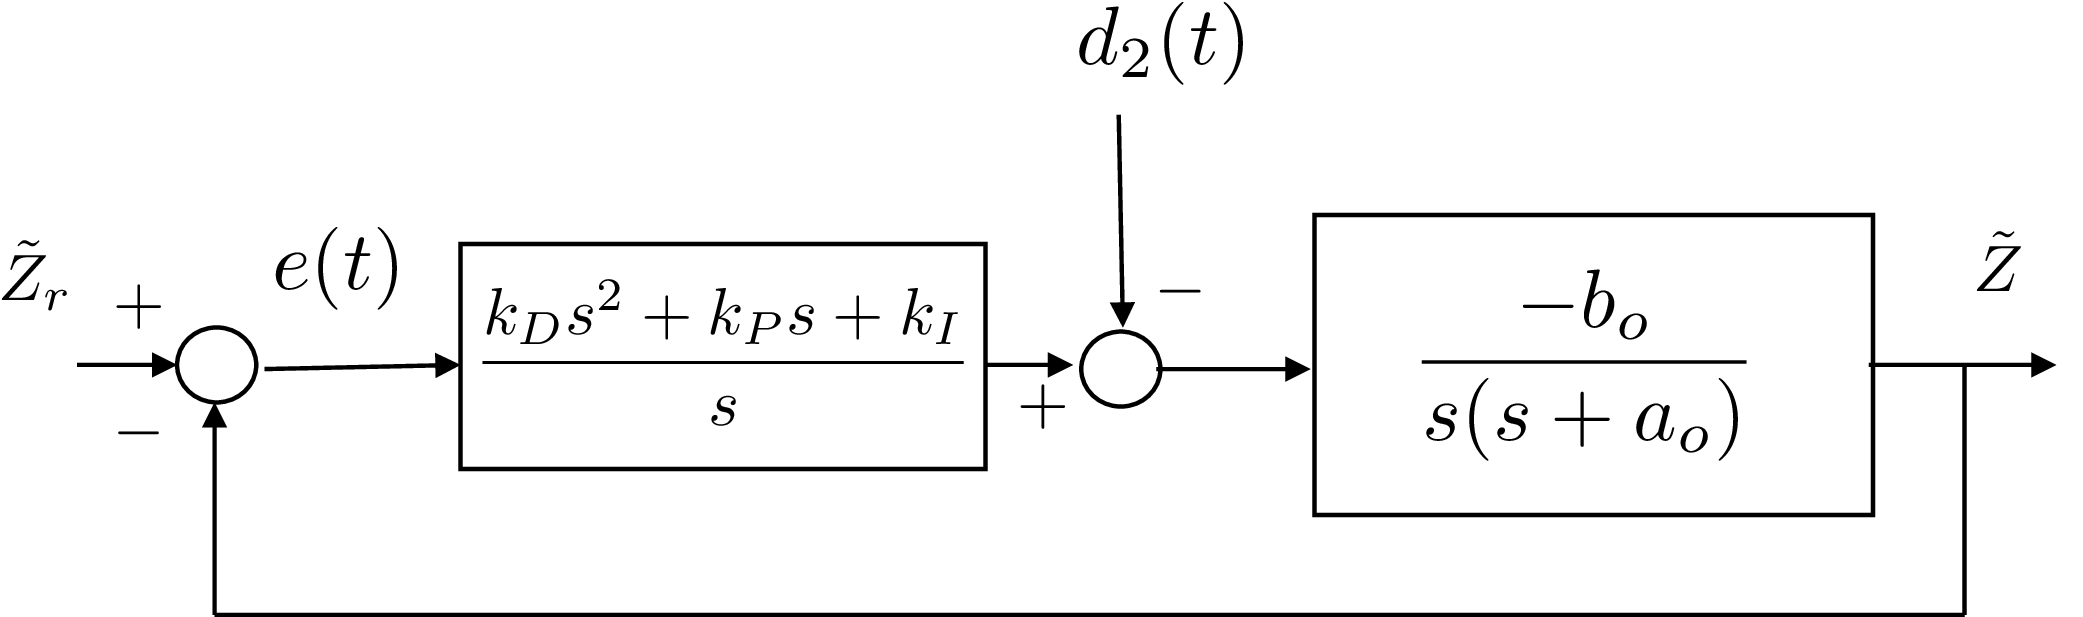
\includegraphics[width=0.8\textwidth]{6_design_studies/figures/hw_vtol_system_type_outer.pdf}
   \caption{Outer loop system for problem HW~\ref{hw:vtol}.\ref{chap:PID-system-type}.}
   \label{fig:hw_vtol_system_type_outer}
\end{figure}
The open loop system is given by
\[
P(s)C(s) = \left(\frac{-b_o}{s(s+a_o)}\right)\left(\frac{k_Ds^2+k_Ps+k_I}{s}\right),
\]
where
\begin{align*}
a_o &= \frac{\mu}{m_c+2m_r} \\
b_o &= \frac{F_e}{m_c+2m_r}.
\end{align*}
When $k_I=0$ there is one free integrator in $P(s)C(s)$ and the system is type~1, and from Table~\ref{table:system_type} the tracking error when the input is a step is 
\[
\lim_{t\to\infty}e(t) = \frac{1}{M_v} = \frac{1}{\lim_{s\to 0} sP(s)C(s)} = -\frac{a_o}{b_ok_P}.
\]
When $k_I\neq 0$, there are two free integrators in $P(s)C(s)$ and the system is type~2.  From Table~\ref{table:system_type} the tracking error when the input is a parabola is 
\[
\lim_{t\to\infty}e(t) = \frac{1}{M_a} = \frac{1}{\lim_{s\to 0} s^2P(s)C(s)} = -\frac{a_o}{b_ok_I}.
\]

For the input disturbance, the transfer function from $D(s)$ to $E(s)$ is given by
\begin{align*}
E(s) &= \frac{P(s)}{1+P(s)C(s)}D(s) \\
     &= \frac{-b_os}{s^3+(a_o-b_ok_D)s^2+(-b_ok_P)s+(-b_ok_I)}.
\end{align*}
When $D(s)= \frac{A}{s^{q+1}}$, the steady state error is given by
\begin{align*}
\lim_{t\to\infty} e(t) &= \lim_{s\to 0} \frac{sP}{1+PC}\frac{A}{s^{q+1}} \\
&= \lim_{s\to 0} \frac{-b_os}{s^3+(a_o-b_ok_D)s^2+(-b_ok_P)s+(-b_ok_I)}\frac{A}{s^q}.
\end{align*}
Without the integrator we have
\begin{align*}
\lim_{t\to\infty} e(t) &= \frac{A}{k_P}
\end{align*}
when $q=0$. Therefore, to an input disturbance the system is type~0, and the steady state error to a constant step of size $A$ on $d(t)$ is $\frac{A}{k_P}$. With the integrator we have
\begin{align*}
\lim_{t\to\infty} e(t) &= \frac{A}{k_I},
\end{align*}
when $q=1$. Therefore, to an input disturbance the system is type~1, and the steady state error to a constant ramp of size $A$ on $d(t)$ is $\frac{A}{k_I}$.


